\documentclass[a4paper]{article}

\usepackage{fullpage} % Package to use full page
\usepackage{parskip} % Package to tweak paragraph skipping
\usepackage{tikz} % Package for drawing
\usepackage{amsmath}
%\usepackage{mathaccent}
\usepackage{hyperref}
\usepackage{subfigure}
\usepackage[utf8]{inputenc}
\usepackage[cyr]{aeguill}
\usepackage[frenchb]{babel}
\usepackage{graphicx}
\usepackage[]{algorithm2e}
\usepackage{xcolor}
\usepackage[]{float}
\title{Compte Rendu - TP ETI5-IMI \\ \textit{Shaders avancés et Marching Cubes}}
\author{Di Folco Maxime - Girot Charly}
\date{27/10/2017}


\begin{document}
\maketitle

\section{Parallax Mapping - Donner l'illusion du relief}

Avant : utilisation de textures \textit{colorées} appliquées directement sur un maillage. Exemple : dessiner un mur de briques comme sur la Fig.\ref{brique}

\begin{figure}[H]
\centering
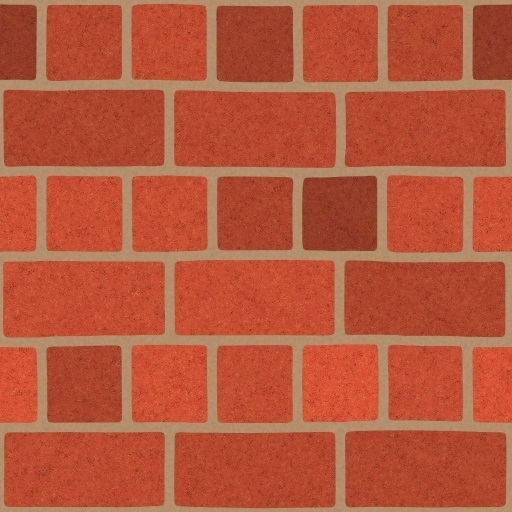
\includegraphics[width=0.3\textwidth]{figures/brick_diffuse.png}\label{briques}
\caption{Images à reconstruire sous la forme d'un panorama}
\end{figure}





\bibliographystyle{plain}
\bibliography{bibliography.bib}
\end{document}